\chapter{PIC architecture}
This chapter describes the architecture of the PIC controller which is used to implement the system.
\section{Introduction to PIC}
We have been given an Explorer 16 development board. The board contains a socket that fits special plug in modules or PIMs. We have also been given two PIMs of the type PIC24FJ128GA010. The type referers to the family: PIC24, subdivision: FJ, available program memory: 128 KB and the model number: GA010. The PIC24 has 16 bit architecture and a lot of built-in modules. Some of the useful modules are UART, SPI, Timers and a Real Time Clock. \\
\subsection{Configuration}
Before any code can be executed on the PIC microcontroller, a series of configuration bits must be set. The categories are seen on figure ~\ref{fig:config}.
\begin{figure}[H]
\centering
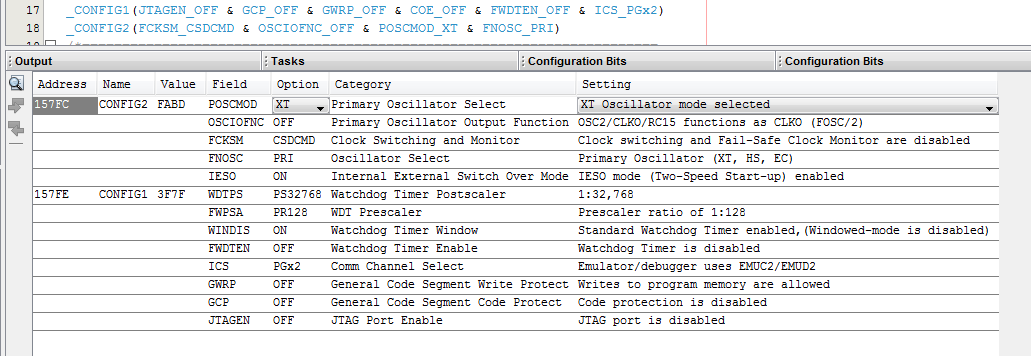
\includegraphics[width=1\textwidth]{billeder/config}
\caption{Configuration bits}
\label{fig:config}
\end{figure} 
\subsection{Difference from known architecture}
We have been working with the AVR Mega32 before. It is also optimised for C-code so a lot of similarities are found. This subsection will explain the differences.\\
A notable difference is names and size of registers. This means that a transition period is needed when wanting to implement basic programmes. Microchip has gone to great lengths to define the registers and the containing bits. An example is found below:
\begin{lstlisting}
IPC0 = 0b0101000000000000;
\end{lstlisting} 
is equal to:
\begin{lstlisting}
IPC0bits.T1IP = 5;
\end{lstlisting} 
This is easier to read while also eliminating the need for writing to the whole register.\\
Another notable difference is that writing to pins are done with latches instead. Writing to a latch is done the following way:
\begin{lstlisting}
LATAbits.LATA5 = 1;
\end{lstlisting}
Reading from a pin is done the following way:
\begin{lstlisting}
x = PORTAbits.PORTA4;
\end{lstlisting}